% !TEX root =  ../supplementary.tex

\section{Parameter Estimates from the Joint Model Fitted to the PRIAS Dataset}
\label{sec:param_estimates_jm_fit_prias}
The posterior parameter estimates for the joint model we fitted to the PRIAS dataset are shown in Table~\ref{tab:DRE_long} (longitudinal sub-model for DRE outcome), Table~\ref{tab:PSA_long} (longitudinal sub-model for PSA outcome) and Table~\ref{tab:DRE_PSA_survival} (relative risk sub-model), and parameter estimates for the variance-covariance matrix $\boldsymbol{D}$ from the longitudinal sub-model are shown in the following Table~\ref{tab:D_matrix}:
\begin{table}[!htb]
\begin{center}
\caption{Estimated variance-covariance matrix $\boldsymbol{D}$ of the random effects ${\boldsymbol{b}=(b_{0d},b_{1d},b_{0p}, b_{1p}, b_{2p}, b_{3p}, b_{4p})}$ (see \ref{subsec:model_def}) from the joint model fitted to the PRIAS dataset. The variances of the random effects are highlighted along the diagonal of the variance-covariance matrix.}
\label{tab:D_matrix}
\begin{tabular}{lrrrrrrr}
\Hline
Random Effects    & $b_{0d}$    & $b_{1d}$    & $b_{0p}$    & $b_{1p}$   & $b_{2p}$   & $b_{3p}$   & $b_{4p}$    \\
\hline
$b_{0d}$ & \cellcolor{black}\textcolor{white}{7.546}  & -0.564 & -0.182 & 0.075 & 0.084 & 0.003 & -0.019 \\
$b_{1d}$ & -0.564 & \cellcolor{black}\textcolor{white}{1.379}  & 0.081  & 0.119 & 0.165 & 0.266 & 0.219  \\
\hline
$b_{0p}$ & -0.182 & 0.081  & \cellcolor{black}\textcolor{white}{0.208}  & 0.031 & 0.034 & 0.068 & 0.014  \\
$b_{1p}$ & 0.075  & 0.119  & 0.031  & \cellcolor{black}\textcolor{white}{0.224} & 0.109 & 0.158 & 0.088  \\
$b_{2p}$ & 0.084  & 0.165  & 0.034  & 0.109 & \cellcolor{black}\textcolor{white}{0.293} & 0.324 & 0.238  \\
$b_{3p}$ & 0.003  & 0.266  & 0.068  & 0.158 & 0.324 & \cellcolor{black}\textcolor{white}{0.480} & 0.312  \\
$b_{4p}$ & -0.019 & 0.219  & 0.014  & 0.088 & 0.238 & 0.312 & \cellcolor{black}\textcolor{white}{0.290}  \\
\hline
\end{tabular}
\end{center}
\end{table}

For the DRE mixed effects sub-model (see Equation \ref{eq:long_model_dre}) parameter estimates, in Table~\ref{tab:DRE_long} we can see that the age of the patient trivially affects the baseline log odds of obtaining a DRE score larger than T1c. In Figure~\ref{fig:fitted_marginal_dre} we present the marginal evolution of probability of obtaining a DRE score larger than T1c, over a period of 10 years for a hypothetical AS patient who is included in AS at the age of 70 years. In addition, we present plots of observed DRE versus fitted probabilities of obtaining a DRE score larger than T1c, for nine randomly selected patients in Figure~\ref{fig:fitted_9subject_dre}.

\begin{table}[!htb]
\begin{center}
\caption{Estimated mean and 95\% credible interval for the parameters of the longitudinal sub-model (see Equation \ref{eq:long_model_dre}) for the DRE outcome.}
\label{tab:DRE_long}
\begin{tabular}{lrrrrr}
\Hline
Variable                         & Mean & Std. Dev & 2.5\%  & 97.5\% & P     \\
\hline
(Intercept)                      & -4.017   & 0.136 & -4.270  & -3.763 & \textless0.000     \\
$(\mbox{Age} - 70)$                      & 0.058    & 0.009 & 0.041  & 0.075  & \textless0.000     \\
$(\mbox{Age} - 70)^2$ & -0.001   & 0.001 & -0.003 & 1.8 $\times 10^{-4}$      & 0.076 \\
visitTimeYears                   & -0.604   & 0.095 & -0.794 & -0.437 & \textless0.000    \\
\hline
\end{tabular}
\end{center}
\end{table}

\begin{figure}[!htb]
\centerline{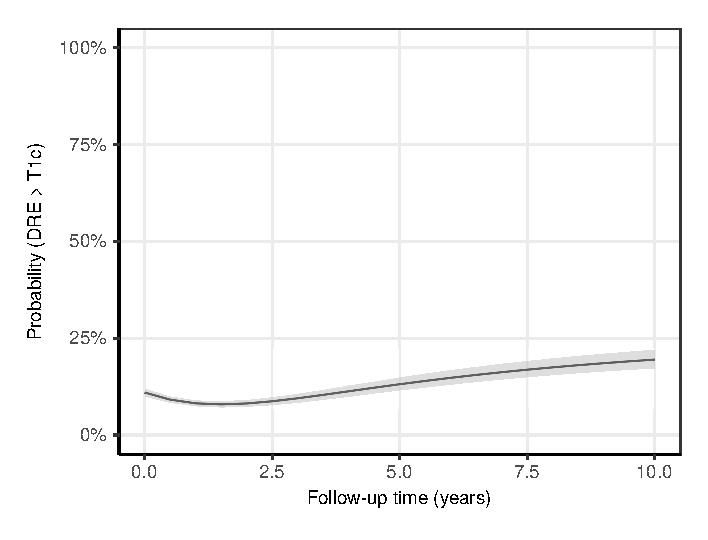
\includegraphics[width=\columnwidth]{images/marginal_dre.eps}}
\caption{Fitted average probability of obtaining a DRE score larger than T1c with 95\% credible interval, over a period of 10 years, for a hypothetical AS patient who is included in AS at the age of 70 years.}
\label{fig:fitted_marginal_dre}
\end{figure}

\begin{figure}[!htb]
\centerline{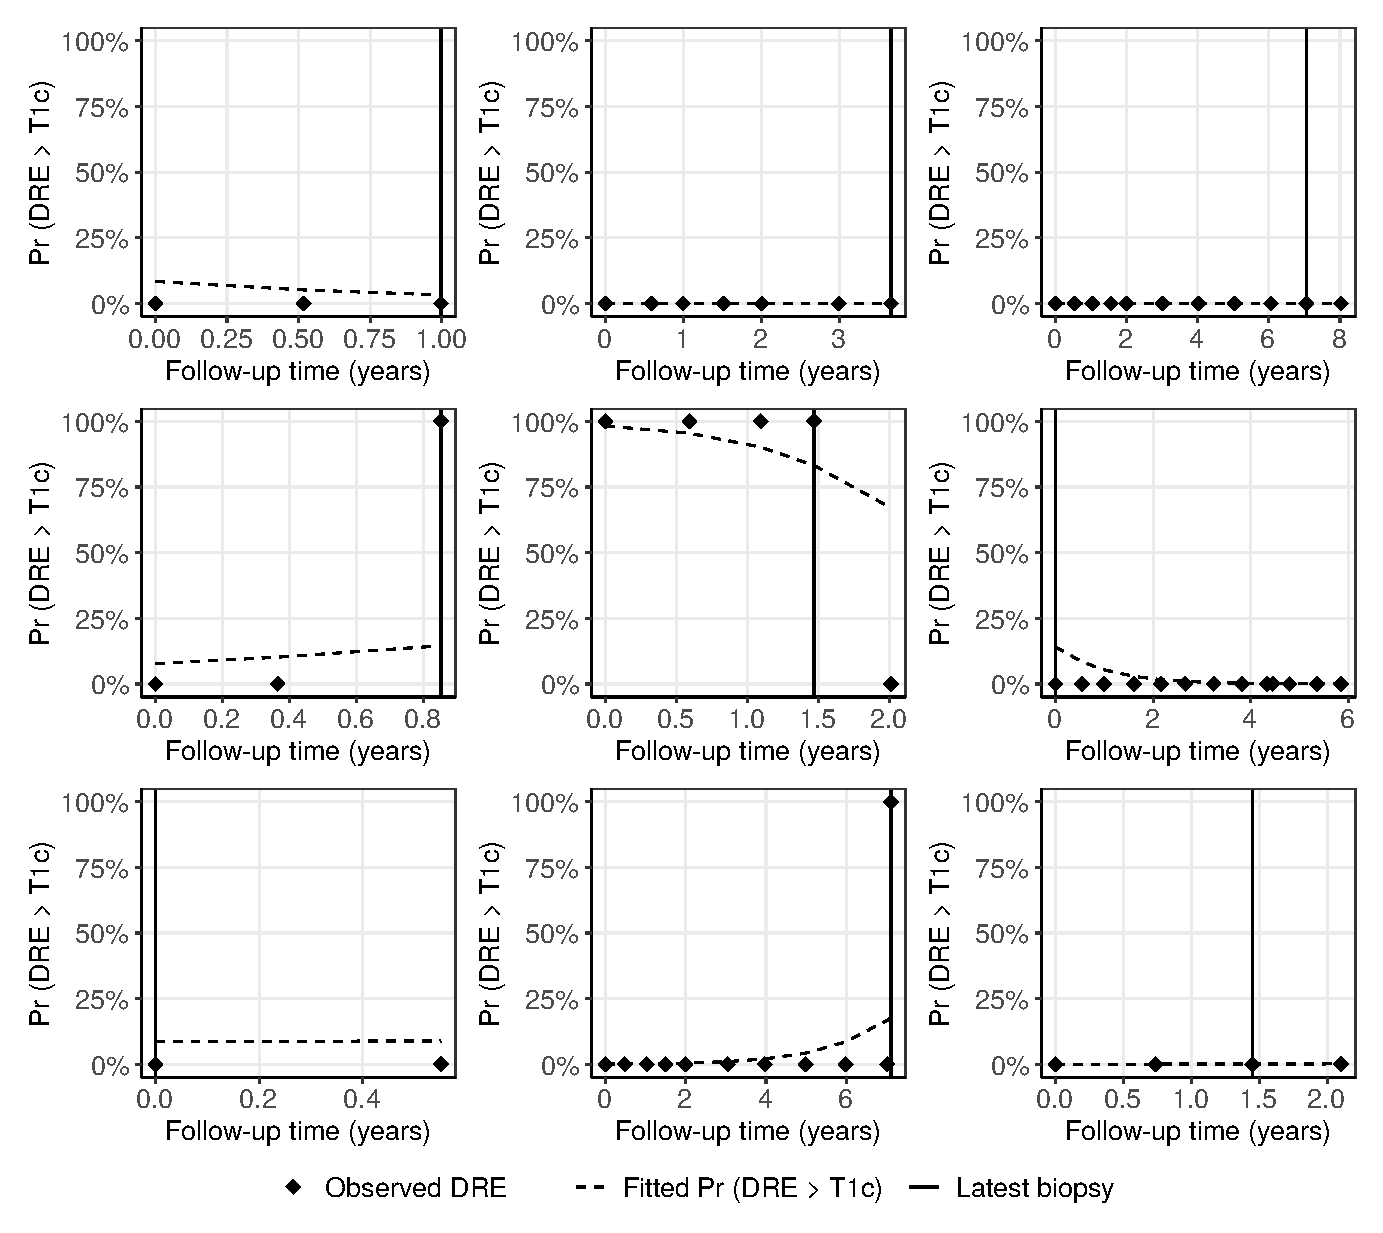
\includegraphics[width=\columnwidth]{images/fitted_9subject_dre.eps}}
\caption{Observed DRE versus fitted probabilities of obtaining a DRE score larger than T1c, for nine randomly selected PRIAS patients. The fitted profiles utilize information from the observed DRE scores, PSA levels, and time of the latest biopsy. Observed DRE scores plotted against 0\% probability are equal to T1c. Observed DRE scores plotted against 100\% probability are larger than T1c.}
\label{fig:fitted_9subject_dre}
\end{figure}

\clearpage

For the PSA mixed effects sub-model parameter estimates (see Equation \ref{eq:long_model_psa}), in Table~\ref{tab:PSA_long} we can see that the age of the patient trivially affects the baseline $\log_2(\mbox{PSA} + 1)$ level. Since the longitudinal evolution of $\log_2 (\mbox{PSA} + 1)$ levels is modeled with non-linear terms, the interpretation of the coefficients corresponding to time is not straightforward. In lieu of the interpretation, in Figure~\ref{fig:fitted_marginal_psa} we present the fitted marginal evolution of $\log_2 (\mbox{PSA} + 1)$ over a period of 10 years for a hypothetical patient who is included in AS at the age of 70 years. In addition, we present plots of observed versus fitted PSA profiles for nine randomly selected patients in Figure~\ref{fig:fitted_9subject_psa}. 

\begin{table}[!htb]
\begin{center}
\caption{Estimated mean and 95\% credible interval for the parameters of the longitudinal sub-model (see Equation \ref{eq:long_model_psa}) for the PSA outcome.}
\label{tab:PSA_long}
\begin{tabular}{lrrrrr}
\Hline
Variable                         & Mean & Std. Dev & 2.5\%  & 97.5\% & P     \\
\hline
(Intercept) & 2.701 & 0.008 & 2.686  & 2.716  & \textless0.000 \\
$(\mbox{Age} - 70)$ & 0.003 & 0.001 & 0.001  & 0.005  & \textless0.000 \\
$(\mbox{Age} - 70)^2$ & -4.7 $\times 10^{-4}$     & 9.8 $\times 10^{-5}$     & -6.6 $\times 10^{-4}$ & -2.7 $\times 10^{-4}$      & \textless0.000 \\
Spline: [0.00, 0.10] years & 0.054 & 0.009 & 0.037  & 0.073  & \textless0.000 \\
Spline: [0.10, 0.70] years & 0.177 & 0.012 & 0.151  & 0.200  & \textless0.000 \\
Spline: [0.70, 4.00] years & 0.194 & 0.016 & 0.161  & 0.225  & \textless0.000 \\
Spline: [4.00, 5.42] years & 0.341 & 0.015 & 0.312  & 0.371  & \textless0.000 \\
$\sigma$ & 0.137 & 0.001 & 0.135  & 0.138  & \\
\hline
\end{tabular}
\end{center}
\end{table}

\begin{figure}[!htb]
\centerline{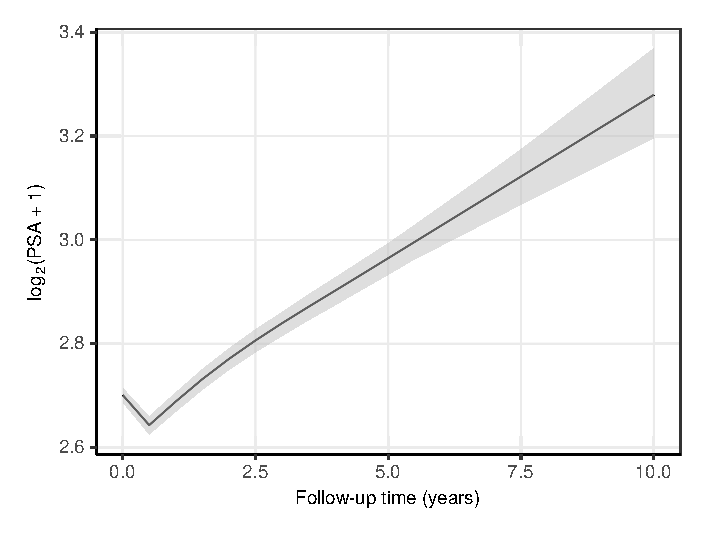
\includegraphics[width=0.7\columnwidth]{images/marginal_psa.eps}}
\caption{Fitted marginal evolution of $\log_2 (\mbox{PSA} + 1)$ levels over a period of 10 years with 95\% credible interval, for a hypothetical patient who is included in AS at the age of 70 years.}
\label{fig:fitted_marginal_psa}
\end{figure}

\begin{figure}[!htb]
\centerline{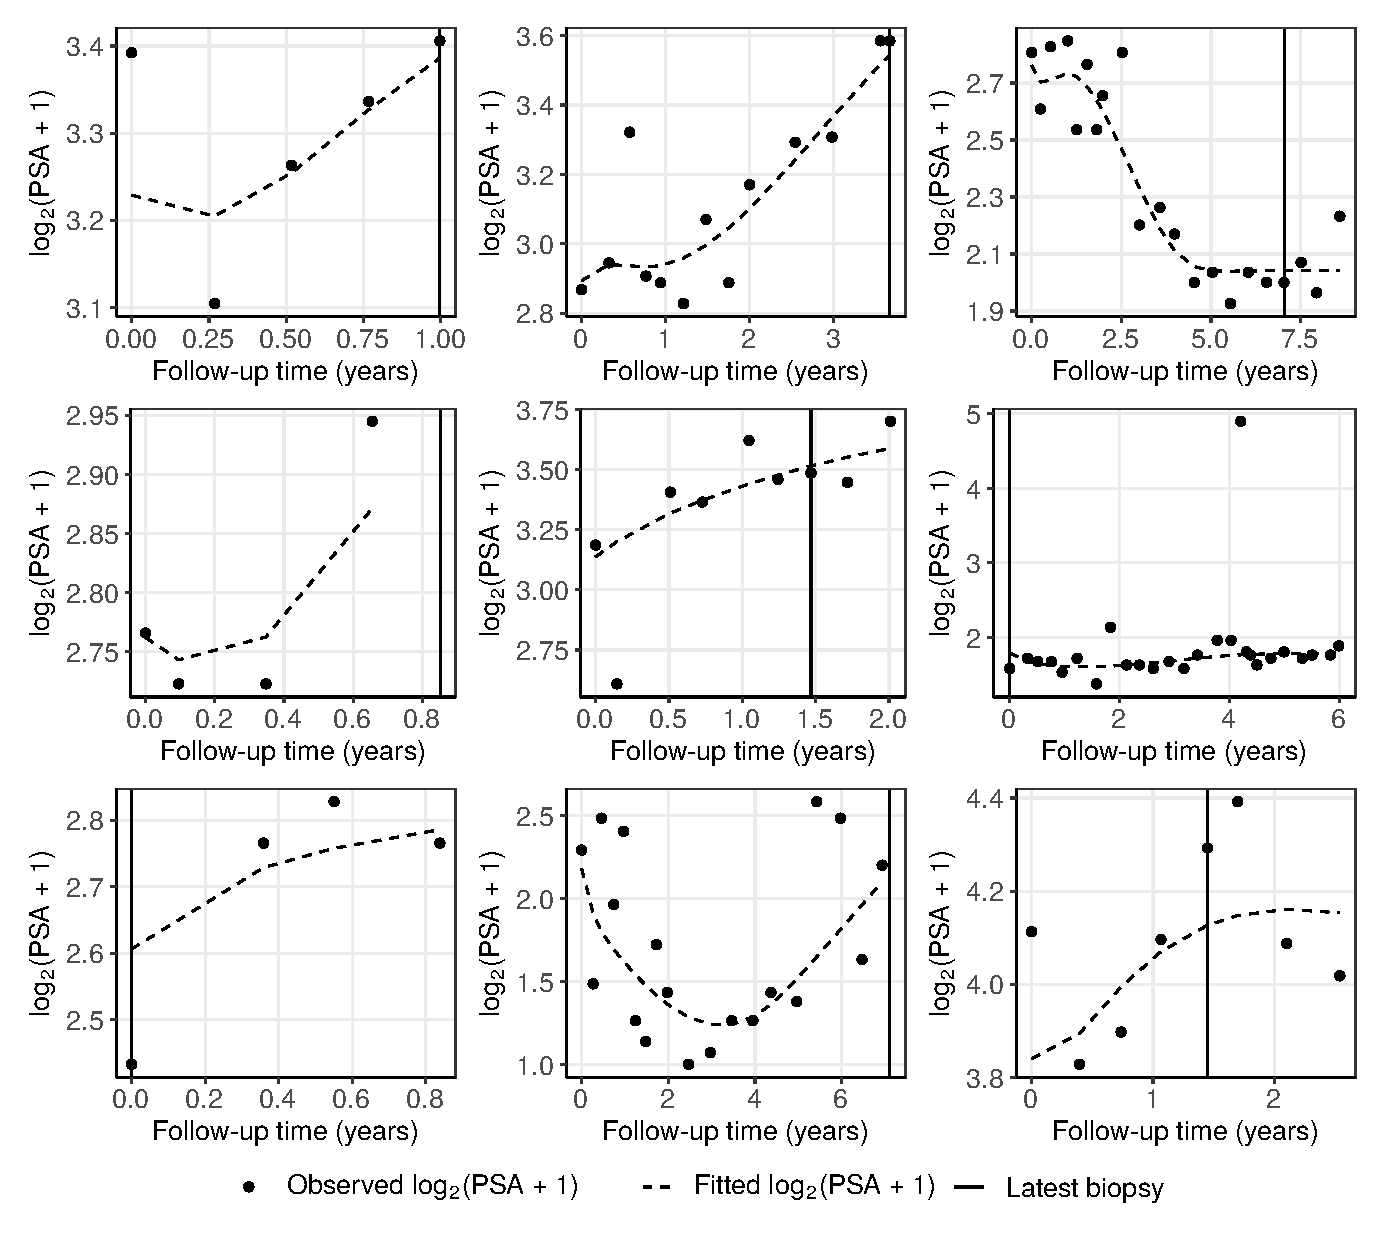
\includegraphics[width=\columnwidth]{images/fitted_9subject_psa.eps}}
\caption{Fitted versus observed $\log_2 (\mbox{PSA} + 1)$ profiles for nine randomly selected PRIAS patients. The fitted profiles utilize information from the observed PSA levels, DRE scores, and time of the latest biopsy.}
\label{fig:fitted_9subject_psa}
\end{figure}

\clearpage

For the relative risk sub-model (see Equation \ref{eq:rel_risk_model}), the parameter estimates in Table~\ref{tab:DRE_PSA_survival} show that both $\log_2 \{\mbox{PSA} + 1\}$ velocity,  and the log odds of having $\mbox{DRE} > \mbox{T1c}$  were significantly associated with the hazard of cancer progression. For any patient, an increase in $\log_2 \{\mbox{PSA} + 1\}$ velocity from -0.03 to 0.16 (first and third quartiles of the fitted velocities, respectively) corresponds to a 1.92 fold increase in the hazard of cancer progression. Whereas, an increase in log odds of $\mbox{DRE} > \mbox{T1c}$ from -6.65 to -4.36 (first and third quartiles of the fitted log odds, respectively) corresponds to a 1.40 fold increase in the hazard of cancer progression. An increase in age at the time of inclusion in AS from 65 years to 75 years (first and third quartiles of age in PRIAS dataset) corresponds to a 1.13 fold increase in the hazard of GR.

\begin{table}[!htb]
\begin{center}
\caption{Estimated mean and 95\% credible interval for the parameters of the relative risk sub-model (see Equation \ref{eq:rel_risk_model}) of the joint model fitted to the PRIAS dataset.}
\label{tab:DRE_PSA_survival}
\begin{tabular}{lrrrrr}
\Hline
Variable                      & Mean   & Std. Dev & 2.5\%  & 97.5\%                 & P              \\
\hline
$(\mbox{Age} - 70)$                      & 0.012    & 0.006 & 2.3 $\times 10^{-4}$ & 0.022  & 0.045 \\
$(\mbox{Age} - 70)^2$ & -0.001   & 0.001 & -0.002 & 1.6 $\times 10^{-4}$      & 0.095 \\
$\mbox{logit} \big\{\mbox{Pr}(\mbox{DRE} > \mbox{T1c})\big\}$                 & 0.147    & 0.017 & 0.115  & 0.183  & \textless0.00     \\
Fitted $\log_2 (\mbox{PSA} + 1)$ value            & 0.104    & 0.078 & -0.044 & 0.256  & 0.193 \\
Fitted $\log_2 (\mbox{PSA} + 1)$ velocity             & 3.396    & 0.564 & 2.376  & 4.475  & \textless0.00   \\
\hline
\end{tabular}
\end{center}
\end{table}

\clearpage

\subsection{Assumption of t-distributed (df=3) Error Terms}
\label{subsec:t-dist-assumption}
With regards to the choice of the distribution for the error term $\varepsilon_{2}$ for the PSA measurements (see Equation \ref{eq:long_model_psa}), we attempted fitting multiple joint models differing in error distribution, namely t-distribution with three, four, and five degrees of freedom, and a normal distribution for the error term. However, the model assumptions were best met by the model with t-distribution having three degrees of freedom, for the error terms. The quantile-quantile plot of subject-specific residuals for the corresponding model in Figure~\ref{fig:qqplot}, shows that the assumption of t-distributed (df=3) errors is reasonably met by the fitted model. 

\begin{figure}[!htb]
\centerline{\includegraphics[width=\columnwidth]{images/qqplot.eps}}
\caption{Quantile-quantile plot of subject-specific residuals from the joint model fitted to the PRIAS dataset.}
\label{fig:qqplot}
\end{figure}

\clearpage
\subsection{Predictive Performance of the Joint Model Fitted to the PRIAS dataset}
To compare the predictive performance of a models having association between hazard of GR and value of longitudinal outcome values, versus a model having the association with both value and velocity, we calculate the area under the receiver operating characteristic curves, also called AUC \citep*{landmarking2017}, for these models (with the only change that $\log_2 \mbox{PSA}$ levels are used as the outcome). Since in a joint model time dependent AUC is more relevant, we calculate the AUC at year one, year two and year three of follow-up in AS. The time window for which the AUC is calculated is one year. The resulting AUC are presented in \ref{tab : AUC}.

\begin{table}[!htb]
\begin{center}
\caption{Area under the receiver operating characteristic curves (AUC), and 95\% confidence interval in brackets. AUC's are calculated for two joint models: first one having association between hazard of GR and longitudinal outcome's value as well as velocity, and second one having association with only longitudinal outcome's value (with the only change that $\log_2 \mbox{PSA}$ levels are used as the outcome).}
\label{tab : AUC}
\begin{tabular}{rrr}
\Hline
Year                      & value and velocity association & value association\\ 
\hline
1 & 0.613 [0.582, 0.632] & 0.595 [0.565, 0.618]\\
2 & 0.648 [0.608, 0.685] & 0.609 [0.568, 0.654]\\
3 & 0.593 [0.560, 0.638] & 0.590 [0.536, 0.628]\\
\hline
\end{tabular}	
\end{center}
\end{table}